%%%%%%%%%%%%%%%%%%%%%%%%%%%%%%%%%
%
%       EXERCÍCIO
%
%%%%%%%%%%%%%%%%%%%%%%%%%%%%%%%%%

\ifdefstring{\atividade}{prova}{%
    \ifdefstring{\modo}{objetivo}{%
        \renewcommand{\valorquestao}{\ValorQObj\ ponto}
    }{%
        \renewcommand{\valorquestao}{\ValorQDisc\ pontos}
    }%
}%

\begin{exercicioBanco}[\valorquestao]
Determine a lei da função \(f\) cujo gráfico está representado abaixo.
\begin{center}
    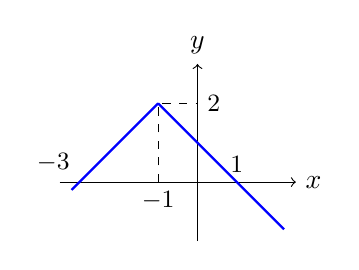
\begin{tikzpicture}[scale=0.5]
        % Eixos
        \draw[->] (-3.5,0) -- (2.5,0) node[right] {\(x\)};
        \draw[->] (0,-1.5) -- (0,3) node[above] {\(y\)};

        % Gráfico da função f(x) = |x+1| - 2
        \draw[domain=-3.2:-1, thick, blue] plot (\x, {(\x + 1) + 2}); % x < -1
        \draw[domain=-1:2.2, thick, blue] plot (\x, {-(\x + 1) + 2});    % x ≥ -1

        % Marcações das raízes (x = -2 e x = 0)
        \node[above left] at (-3,0) {\small\(-3\)};
        \node[above] at (1,0) {\small\(1\)};

        % Marcação do vértice (x = -1)
        \draw[dashed] (-1,0) -- (-1,2) -- (0,2);
        \node[below] at (-1,0) {\small\(-1\)};
        \node[right] at (0,2) {\small\(2\)};
    \end{tikzpicture}
\end{center}

% Define as alternativas
\newcommand{\alternativas}{%
    \begin{center}
        \begin{tabularx}{\textwidth}{XXXXX}
            (a) \(|x - 1| + 2\). &
            (b) \(|x + 1| + 2\). &
            (c) \(-|x - 1| - 2\). &
            (d) \(|x - 1| - 2\). &
            (e) \(-|x + 1| + 2\).
        \end{tabularx}
    \end{center}
}

% Define a resposta correta
\newcommand{\resposta}{E}

% Lógica condicional para exibição
\ifdefstring{\atividade}{lista}{%
    \alternativas
    \vspace{0.5em}
    
    \noindent\textbf{Resposta:} letra \textbf{\resposta}.
}{%
    \ifdefstring{\modo}{objetivo}{%
        \alternativas
    }{%
        % modo = discursiva → não mostra alternativas
    }
}
\end{exercicioBanco}

